% Created 2015-02-27 Fri 21:00
\documentclass[11pt]{article}
\usepackage[utf8]{inputenc}
\usepackage[T1]{fontenc}
\usepackage{fixltx2e}
\usepackage{graphicx}
\usepackage{longtable}
\usepackage{float}
\usepackage{wrapfig}
\usepackage{rotating}
\usepackage[normalem]{ulem}
\usepackage{amsmath}
\usepackage{textcomp}
\usepackage{marvosym}
\usepackage{wasysym}
\usepackage{amssymb}
\usepackage{hyperref}
\tolerance=1000
%\usepackage{lmodern}
\usepackage{algorithm2e}
\usepackage{times}
\usepackage[usenames,dvipsnames]{xcolor}
\hypersetup{colorlinks=true, citecolor=Blue, linkcolor=Black, urlcolor=Blue}
\author{Hermann Pauly}
\date{}
\title{A wrapper for \emph{segemehl} output}
\hypersetup{
  pdfkeywords={},
  pdfsubject={},
  pdfcreator={Emacs 24.4.1 (Org mode 8.2.10)}}
\begin{document}

\maketitle
\begin{abstract}
Alternate splicing is a cellular process that massively increases the amount of transcripts
encoded in a single gene. Apart from commonly spliced mRNAs from single genes, different splicing
variants, both functional and pathological, have been observed. The NGS mapping software
\emph{segemehl} maps multi strand fusion and circular transcripts, but offers no method to
visualise them yet. Here I present a software to automatise selective visualisation of 
\emph{segemehl} data files. I applied it to sequenced and processed skin cell data and found 
numerous multi strand fusion transcripts with low abundancies each.
\end{abstract}



\section{Introduction}
\label{sec-1}

Alternate splicing is a cellular process that massively increases the amount of different RNA
and proteins available to organism without the need to store more genetic information. 
The variability is achieved by cutting gene transcripts at defined splice-sites and fusing
desired parts to different functional mRNAs.
Next to gene silencing and methylation, alternate splicing is another mechanism that allows 
cells to differentiate.
On the other hand, erroneous splicing events can cause various diseases, thus making their
understanding crucial to genomic research.

According to Hoffmann et al. \cite{smpaper}, data from NGS sequencing however has shown, that not
all splice events connect exons from a single gene to a regular mRNA, and not all seemingly
aberrant splicing needs to be pathologic.
Splicing can connect both ends of an RNA strand so it forms a circular RNA, which may have
regulatory roles. 
In some cases and organisms also the fusion of RNA transcribed from different strands of a 
chromosome or even from different chromosomes could be observed.

To analyse genomic data, in the past, we were limited to low-throughput sequencing methods like
Sanger sequencing.
However, the next generation sequencing (NGS) methods of nowadays enable us to obtain near 
complete quantitative and qualitative genomic snapshots of cell states in a single go with very 
high accuracy.

Such proceedings typically produce huge amounts of short RNA sequence fragments at base-pair 
level accuracy.
To further analyse - or visualise - these datasets, it is neccessary to recompile proper 
fragments and reassemble the RNAs they stem from, thus reconstructing the whole transcriptome.
Three assembly strategies are commonly followed: \emph{ab initio} assembly based on a reference 
genome, \emph{de novo} assembly and methods combining both.

\emph{De novo} assemblers usually work by constructing De Bruijn Graphs, that is graphs grouping
sets of overlaps. The \emph{Rnnotator, Multiple-k}, and \emph{Trans-ABy-SS} softwares construct multiple
De Bruijn graphs and postprocess them to reassemble contigs. Other assemblers like \emph{Trinity}
and \emph{Oases} reassemble RNAs and isoforms directly from single De Bruijn graphs.
\emph{De novo} assembly does not require reference genomes, so it can be applied to organisms for
which no complete genome sequencing has been done yet. As it only works on transcribed RNA,
it cannot be confused by long, ambiguous, or unconventional DNA intron sequences.

\emph{Ab initio} assemblers rely on existing reference genomes for their task. They align all
fragments to the reference genome, create graphs of overlapping fragments and then traverse
the graphs to reconstruct isoforms either by statistical (\emph{Scripture}) or by pathfinding 
(\emph{Cufflinks}) methods.
To align fragments to genome, two methods are common.
Burrow Wheeler Transform finds all suffix combinations of a string and thus allows to
match strings with few differences very quickly, finding all combinations of possible matches.
Seed-and-extend algorithms search exact matches for parts of their input strings and try to
extend them along the genome with Smith-Waterman methods, thus allowing parametrisation of the
scoring. They tend to match around known splice sites.
These reference-based techniques can split down assembly problems and thus work on lower powered
machines, they can match fragments with low abundancy, bridge sequencing gaps, and discard 
sequencer artifacts (which will not match the genome very well in any place) (compare 
\cite{martin2011}).

\emph{Segemehl} is a reference-based NGS mapping utility following a seed-and-extend approach. It
deliberately omits searching for known splice sites to be able to find circular RNAs and new 
kinds of \emph{fusion transcripts}, transcripts that stem from distant loci of different strands of a 
chromosome, or fusions of RNA transcribed from multiple chromosomes. In this work the latter two
events are termed multistrand events.

Here I present the foundation for a software that visualises the output of \emph{segemehl} mapped
sequencing data.


\section{The program}
\label{sec-2}

My goal was to develop a software that is able to create visualisation plots for RNA mappings 
from \emph{segemehl} processed files in an automated way.
It should be able to visualise "standard" RNAs, with exons originating from a defined area on a 
specific chromosome, as well as novell kinds of transcripts detected with the \emph{segemehl} method. 
As NGS methods produce large data files, it had to be fast and needed to store the results 
efficiently in RAM while running. 
Due to the large numbers of RNA transcripts that are typically processed in NGS machines,
user-definable selection of output needs to be implemented.
I chose the following filtering options:
detection of all multistrand RNAs,
detection of all circular RNAs,
and all isoforms containing user-defined chromosome and position pairs.
Future versions also aim to further refine the search by allowing to filter by link depth, that
is the number of times a connection of any two splits within transcripts and isoforms occured in 
the input files.
The software should abstract the temporary representation, input and output backends, so future 
versions can be extended to work with other mapping tools' output files and customise resulting 
file formats and visual appearance.


\subsection{Overview and used third-party software}
\label{sec-2-1}

The visualisation program with the working title \emph{chipboard} is written in \emph{C++} for a balance
of speed and memory efficiency on the one hand, and safe and readable code on the other hand.
I automated compiling by using the \emph{cmake} build managing system(\cite{cmake}). For GUI creation,
I used \emph{Qt4.8} (\cite{qtpage}).
For development I used the \emph{gcc} compiler suite v4.8.2 and \emph{cmake} v3.1.0.


\subsection{Plot types}
\label{sec-2-2}

\subsubsection{Isoform tree plots}
\label{sec-2-2-1}
\label{txt:tree1}

In an effort to increase the information content and readability within plotted RNAs with
multiple isoforms, I decided to visualise RNA not as a linear strand with connection lines (see
fig. \ref{fig:linearrna}), but as a tree structure. Split reads are nodes, with their basepair
lengt reflected in the node length, while splicing events are edges, allowing a more
intuitive understanding of existing isoforms.


\begin{figure}[htb]
\centering
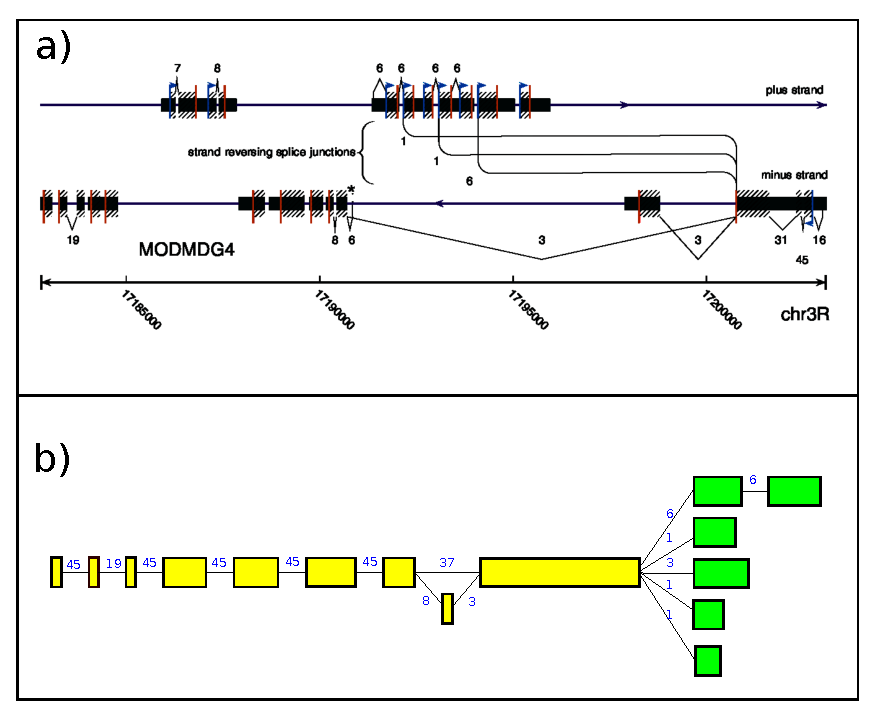
\includegraphics[width=.9\linewidth]{./rnas.eps}
\caption[Tree-like RNA visualisation]{The same information displayed \textbf{(a)} in a traditional linear presentation and \textbf{(b)} in a treemap mockup (note that the reverse strand is presented in another colour, as it will be detected differently by \textit{segemehl}}\label{fig:linearrna}
\end{figure}

%\begin{figure}
% \centering
% 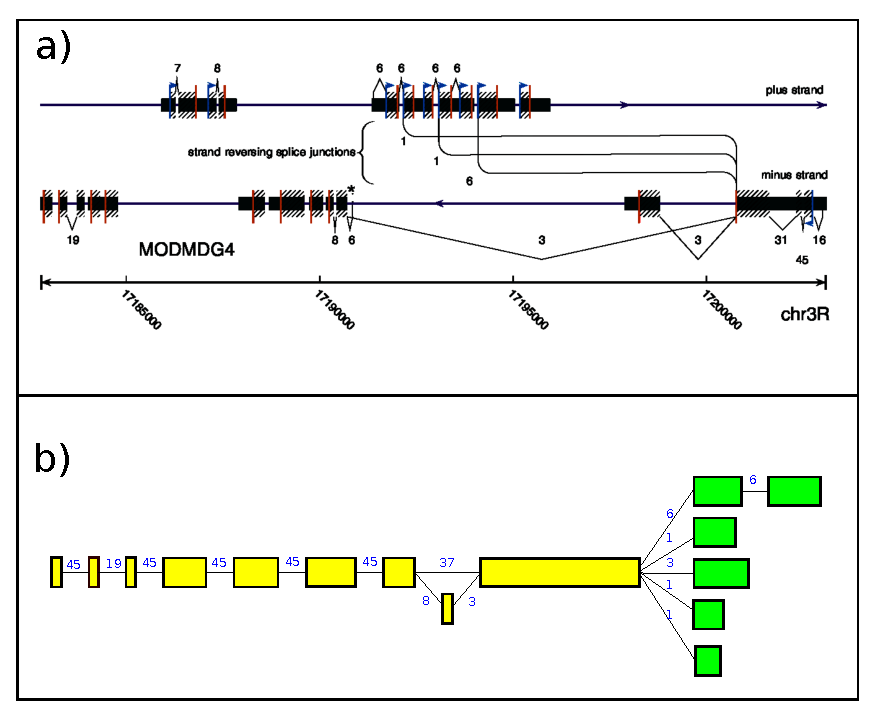
\includegraphics[width=0.8\textwidth]{rnas}
% \caption[Tree-like RNA visualisation]{The same information displayed \textbf{(a)} in a traditional linear presentation and \textbf{(b)} in a treemap mockup (note that the reverse strand is presented in another colour, as it will be detected differently by \textit{segemehl}}\label{fig:linearrna}
%\end{figure}


\subsubsection{Circular plots}
\label{sec-2-2-2}
\label{txt:circ1}

Circular RNA will be visualised as ring structures. The size and angle of ring fragments for each
split indicate its relative length, compared to the whole ring.


\subsection{Reassembly of \emph{segemehl} split reads}
\label{sec-2-3}
\label{txt:reassembly}

\emph{Segemehl} with its \emph{split} option enabled divides input RNA reads into fragments, maps each 
of those split fragments to the chromosomes and position it fits best and stores them, 
line-wise and in order, inside the \emph{sam} file, together with information how it had
performed the splitting and mapping.
It thus provides a guideline how to reassemble the input reads.
With each split the following information is stored: 
(1) the chromosome, read position, and read direction ("strandiness") it was mapped to,
(2) information about mapping length and quality,
(3) a number specifying the order of splits along the original read,
(4) information about chromosome, position and strandiness of the previous and next split in
this read, if there are any (see \cite{smmanual}).

For reassembly I treat reads as doubly $n/m$-linked directed, acyclic graphs, where nodes
resemble exons and edges resemble splicings.
Each node stores the length in base pairs and the chromosome of origin of the split it 
represents, as well as edges resembling detected 3' and 5' splice events.
The chromosomes are represented as ordered maps, which map 3' and 5' positions to the respective
nodes (compare fig. \ref{fig-datastructure}) to achieve $O(\log n)$ lookup times.
By continuous adding nodes to existing subgraphs, the sequencer read fragments get reassembled
to full RNAs, with all their isoforms encountered merged into a single graph.


\begin{figure}[htb]
\centering
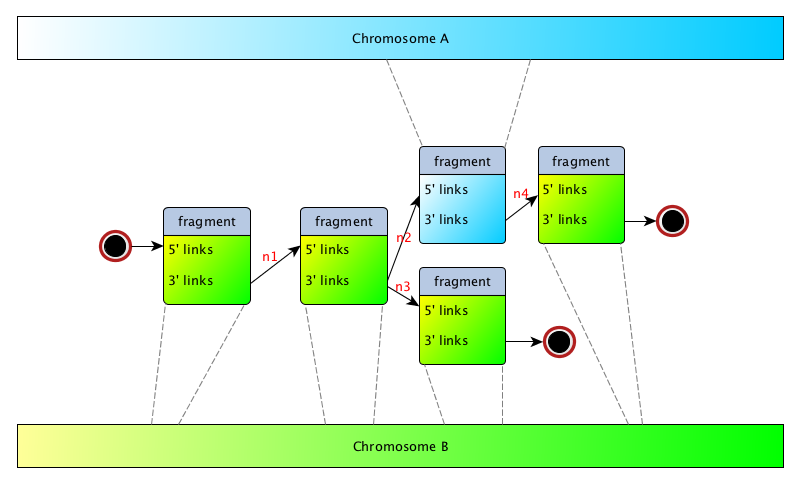
\includegraphics[width=.9\linewidth]{./datatype.png}
\caption[\textit{chipboard}'s internal datastructure]{\textit{chipboard}'s internal datastructure. Graph nodes resemble split fragmens/exons and edges resemble splicings. Chromosomes are resembled as ordered maps of node-pointers to allow for quick selection.}\label{fig-datastructure}
\end{figure}


\subsubsection{Reassembling the original RNA sequences}
\label{sec-2-3-1}

Following \emph{segemehl}'s philosophy according to Hoffmann et al. \cite{smpaper}, I did not test for
meaningfulness of splice sites. I used the information I had extracted (see \ref{txt:reassembly})
to reassemble the original inputs by a series of simple steps on every line of \emph{.sam} data:
First the program determines the chromosome positions the 5' and 3' ends map to. As
\emph{segemehl} does neither fill in the "match length" property nor the match position of the 5' end,
the program reconstructs them from the \emph{cigar} string, which encodes assumed matches, mismatches,
insertions and deletions in the mapping process (see \cite{samFormat}). 
Next, the program compares the resulting chromosome positions with existing nodes' data and 
creates a new node if no matching one exists.
Then the program looks, if the current split's 3' and 5' ends are linked to other splits. If
there are any linked splits, a check for existing modes is done. Existing nodes are doubly-linked
immediately. If a split's upstream predecessor is linked, the predecessor's link depth counter
to the current split is increased. As \emph{segemehl} writes all encountered fragments in order, this
is assured to find correct link depths. If the \emph{.sam} file has been sorted or modified after 
the \emph{segemehl} processing, link depths may not be counted correctly, but due to the usage
of doubly linked nodes, all isoforms from the original input file will be reconstructed.
Assuring correct link depths in randomly ordered input files is possible if the input file gets
processed twice, but was considered impractical standard behaviour, as it would double the 
relatively long runtime.


\subsubsection{Detecting multistrand reads}
\label{sec-2-3-2}

One of the key features of \emph{segemehl} is the mapping of read fragments to different chromosomal
strands of origin. To detect such multistrand chromosomes on user request, the information from
\ref{txt:reassembly} is applied straightforward: if a split's successor is on a different
chromosome, the respective split is added to a list of multistrand seeds, which can be expanded
to a full isoform tree (see \ref{txt:tree1}) for plotting on the available backends.


\subsubsection{Detecting circular reads}
\label{sec-2-3-3}

Another feature of \emph{segemehl} is the detection of circular RNAs.
The split segments of a linear RNA read follow each other in a definite order in the resulting
\emph{.sam} file. This can be seen in both an ascending ordering number and an ascending position on
the chromosome (or descending in case of reverse direction). A circular transcript can
be identified by an ascending order number combined with a position which lies upstream the
chromosome position of a split with lower read number (with respect to the reading direction).
A split with these properties gets added to a list of circular seeds, to be expanded to full
circular graphs (see \ref{txt:circ1}) if the user requests circular detection.


\subsection{Plotting}
\label{sec-2-4}
\label{txt:bfs}

In \ref{txt:tree1} and \ref{txt:circ1} I indicated, that only single splits of subgraphs
interesting to the user get saved to a list for later expansion to full (sub-)graphs.
There were two reasons for the decision to save graph seeds instead of full graphs:
(1) memory consumption was a huge concern during development, and
(2) as there is no way to find out, when all copies and isoforms of a read have been processed,
a full copy of each graph would have to be updated every time another read adds to it.
Thus only one node of the interesting graph is saved and expanded with a breadth-first traversal
of its linking edges, as seen in algorithm \ref{alg:bfs}.
Note that this approach evaluates the full subgraph of nodes connected to the seed, which may
also contain nodes that share no primary connection to it, e. g. are an isoform of an exon that
exists only in some isoforms of the queried graph, but never occur in combination with the query
seed.
No filtering of possibility or probability of isoforms is applied.
There is no immediate drawing done, the method generates coordinates which can then be handled
or modified by the drawing backend.

The drawing backend encodes basepair length in the size of the resulting fragments, chromosome
association in colours, and displays link depth numerical.

\begin{algorithm}  \label{alg:bfs}
  \DontPrintSemicolon
  \KwIn{$node$: one node of a graph}
  \KwOut{The whole graph which is connected to $node$}
  $q$ $\leftarrow$ empty queue\;
  push $node$ to $q$\;
  \While{$q$ not empty}{
    $N$ $\leftarrow$ pop first element from $q$\;
    mark $N$ as visited\;
    create a visualisation node for $N$\;
    \lForAll{unvisited 5' links $el5$ in $N$}{
      push $el5$ to $q
    }
    \ForAll{3' links $el3$ in $N$}{
      create a visualisation edge $N \to el3$ with link depth label\;
      \lIf{$el3$ unvisited}{
        push $el3$ to $q$
      }
    }
  }
  \caption[BFS graph seed traversal]{Breadth first traversal (BFS) to expand a complete graph from a single member node}
\end{algorithm}

\subsubsection{Isoform trees}
\label{sec-2-4-1}
\label{txt:tree2}

The tree visualisation is generated from the coordinates generated by algorithm \ref{alg:bfs}.
Starting from the first node without links on the 3' end drawn at the leftmost x position, 
the nodes are drawn. Depending on the number of nodes linked to a node's 5' end, those 5'-linked
nodes get drawn recursively with an offset in y-position (compare algorithm \ref{alg:tree}).


\begin{algorithm}
\label{alg:tree}
\DontPrintSemicolon
\KwIn{$node$, x-coordinate $x$, y-coordinate $y$}
\KwResult{Draw tree graph representation}
\BlankLine
\emph{Start with $node =$ node without predecessors, $x=0, y=0$}
\BlankLine

\SetKwProg{Fn}{function}{:}{end}
\Fn{naiveLayout($node, x, y)}{
  draw $node$ at position ($x, y$) \;
  $nextX \leftarrow x + 1$ \;
  $y0 \leftarrow -$(number of 5' links $ / \; 2)$\;
  \For{$i \leftarrow 0$ \KwTo number of 5' links}{
    $nextY \leftarrow y0 + i$ \;
    $nextNode \leftarrow$ 5'links[i]\;
    draw edge to $(x+1, nextY)$ \;
    naiveLayout(nextNode, nextX, nextY)
  }
}
\caption[Naive tree layout]{Naive tree layout. More complex graphs may create colliding coordinates for nodes}
\end{algorithm}


\subsubsection{Circular reads}
\label{sec-2-4-2}
\label{txt:circ2}

The basepair length of each split is compared to the basepair length of the complete circular RNA
to determine which fraction of the ring will be assigned to it.
This method does not treat the special case of a circular graph with isoforms properly.



\subsection{Image export}
\label{sec-2-5}

At the moment, only the export of programmatically generated Adobe Encapsulated PostScript (\emph{.eps})
is supported, but the program is designed to ease implementation of drawing backends.
As another option, the reconstructed and filtered graphs can be exportet to \emph{GraphML} format
for visualisation with 3rd party software.

\clearpage

\section{Results}
\label{sec-3}


\subsection{Test cases}
\label{sec-3-1}
\label{txt:test}

\begin{wrapfigure}{l}{0.5\textwidth}
\centering
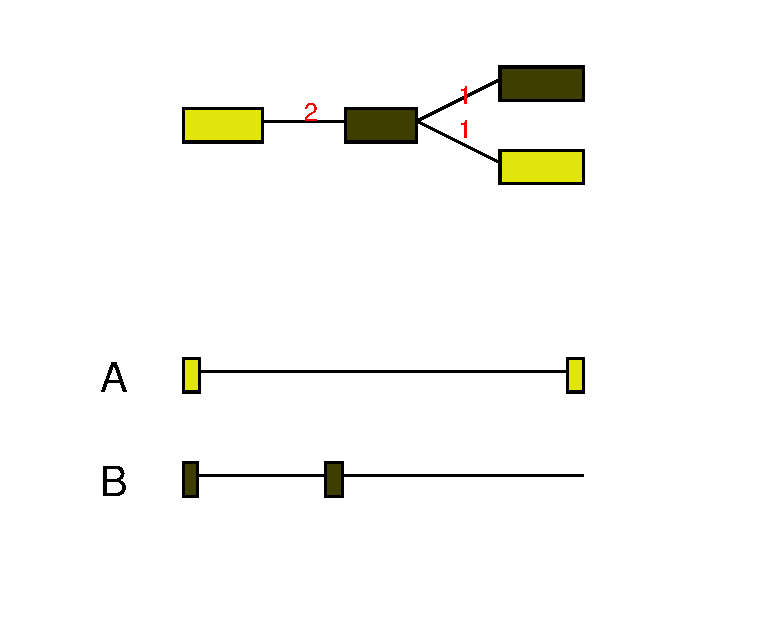
\includegraphics[width=0.48\textwidth]{./tree2.eps}
\caption[Multistrand tree plot of test data]{Treeplot of RNA that contains multistrand events and two isoform, generated from test data.}\label{fig-tree}
\end{wrapfigure}

To create test cases, I used a custom \emph{python} script which simulates chromosome data through
randomly drawing from the nucleid base letters $[A,C,G,T]$ and writing them into a \emph{.fasta} file.
From these simulated chromosomes, I copy-pasted segments into another \emph{.fasta} file to simulate
sequencer reads. Then I used \emph{segemehl} to remap the simulated reads to the simulated chromosomes.
This allowed me to know the desired results and quickly spot errors during development.

When I allowed \emph{segemehl} to split input reads and map the fragments to different chromosomes 
(multistrand reads), it found the origins of all fragments correctly. However, when read length
exceeded 120 bases, \emph{segemehl} often crashed with memory access errors.

Visualisation of output files with \emph{chipboard} worked well with multistrand RNAs that have only 
a small number of isoforms (see fig. \ref{fig-tree}).
More complicated transcripts will result in skewed output, however, as nodes farther down in the
tree may have multiple 5'links themselves, thus changing their respective y coordinate offset in
ways that collide with sibling nodes' positions.


\subsection{Real world data}
\label{sec-3-2}
\label{txt:data}

To test \emph{chipboard} on real world data, I successfully ran it on 41 - 69GB files from 
\cite{skinpaper}, where it detected millions of multistrand RNAs per file. Sampling of generated
output files showed that detected strand-switching events tend to be short (2-3 exons) and have a
low link depth (never above 4 in 20 randomly picked output images), see fig. \ref{fig-tree2} for 
an example. Full evaluation of all found events was not done.

The available data has been pre-filtered for poly-A reads, so circular transcripts are not 
contained, as poly-A tails are signalling structures of valid linear mRNA.
Hence the search for circular transcripts was not enforced.

\begin{wrapfigure}{l}{0.5\textwidth}
\centering
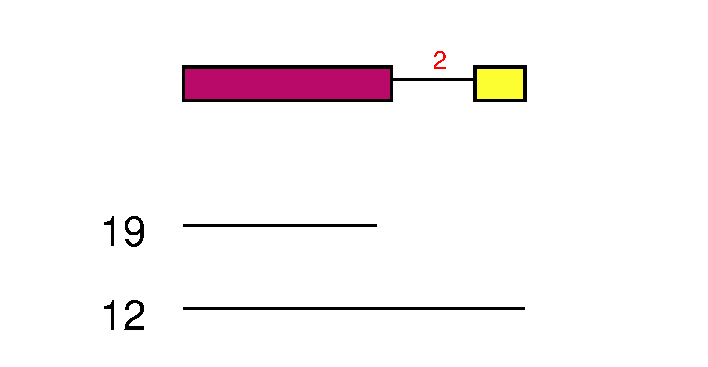
\includegraphics[width=0.5\textwidth]{./real.eps}
\caption[Multistrand tree plot of real data]{Treeplot of a multistrand split event found in real dataset. Short RNA consisting of a 100-base fragment from chromosome 19 and one 24-base fragment from chromosome 12, found twice in the dataset.}\label{fig-tree2}
\end{wrapfigure}


\subsection{Performance}
\label{sec-3-3}

\begin{figure}[htb]
\centering
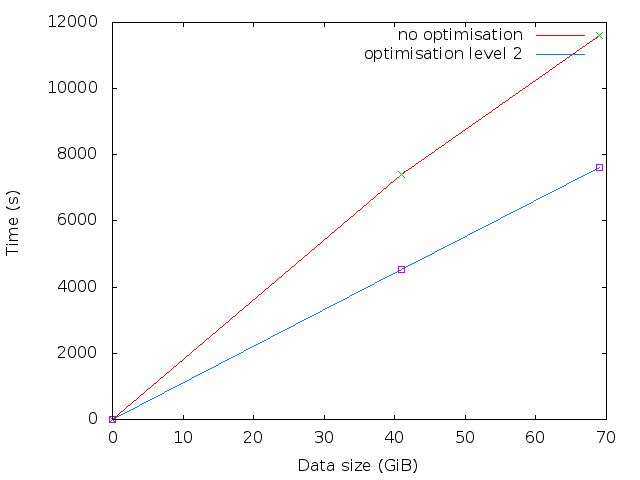
\includegraphics[width=.9\linewidth]{./times.png}
\caption[Runtime comparison]{Runtime comparison on \textit{rhskl5} workstation. Runtime increases in linear fashion with data size, while optimised code runs 1/3 faster. Times were taken for 57 MiB, 41 GiB and 69 GiB files.}\label{fig:times}
\end{figure}


Running on datasets of different size, \emph{chipboard} showed linear ($O(n)$) runtime.
On the \emph{rhskl5} workstation of Universität Regensburg, about 20GB of data could be processed per
hour without optimisation flag; setting the optimisation to level 2 (\texttt{-O2}) increased the
performance to 32 GB/h (see fig \ref{fig:times}).
Profiling showed, that 50\% of the runtime is spent tokenizing text strings from the
human-readable \emph{.sam} input files to parse them for data.


\clearpage

\section{Discussion}
\label{sec-4}

The software \emph{chipboard} is a tool to visualise NGS sequencing data which has been mapped with
the \emph{segemehl} tool. It allows to scan for RNA assembled of exons from different chromosomes 
and is at the time of writing the only software known to the author that automates the 
visualisation of such events.
In addition, it allows the user to select RNA which contains exons from specific chromosome
positions. With tree-like isoform graphs, it tries to increase visual information content in 
comparison with more common visualisation approaches.
Filtering for possible of probable event is omitted; \emph{chipboard} shows the raw findings of
\emph{segemehl} directly.

In its current state, \emph{chipboard} is stable but not complete. Detection and visualisation of
circular graphs has been deactivated in the current build, as it is only rudimetary and not
yet thoroughly tested. Also, as hinted in \ref{txt:circ2}, circular RNAs with splice variants can be
ambiguous. When traversing the graph, the program could get stuck in a non-circular isoform. To
avoid this, some shortest path search like Djikstra's algorithm could be applied to find a
complete path from the start-node to the end node.

The visualisation of tree graphs works satisfyingly for simple graphs with a low number of isoforms.
RNAs with many complex isoforms will create graphs with overlapping node coordinates. To adress
this, a full-fledged graph layout algorithm must be used. I suggest to refrain from force-based
methods in favour of hierarchy-based methods like Sugiyama's method.
Although force-based approaches create graphs which are tendentially more aesthetically
pleasing, their average runtime is far higher (see \cite{hbgraphs}).

Although the processing speed of 32GB per hour seems quite moderate, some optimisation is still desirable.
When parsing the \emph{.sam} input files, it is impossible to predict, which split will be read next,
and what graph it may belong to. This makes parallellization very hard. Mutexes could be used
to lock all nodes of a graph for a single process, but this would include traversing up to two
complete graphs for every split that is added, plus the time needed to wait for other processes
releasing locks, so no critical speed gain should be expected from this.
However, when running the program, about 50\% of the runtime is used tokenizing string data. This
is done serially, so a dual-thread approach could be used, where one thread tokenizes strings and
pushes them to a thread-safe dequeue buffer, while a second thread pops the tokenized strings and
constructs the graphs from them. This way, it should be possible to process the same data in half
the time.

To improve the usefulness of \emph{chipboard}, visualisation should be extended in various ways.
Unused regions of the chromosomes, against which splits are mapped, should be shortened in the
graphical output. Chromosome position numbers  should be displayed, and the splits in the output
graphs should display identifiers to allow connecting them to their respective exon regions.
Also a method to list all findings of interest in a text file for further processing would prove
a usefull addition and should be trivial to implement.

The analysis of real world data (\ref{txt:data}) showed numerous findings of strand-switching
events in RNA synthesis, but due to the short length and low link depth found in subsamples the
reliability of those findings must be doubted. The samples seem to imply sequencer artifactcs 
rather than real discoveries, but to make any reliable statements, proper statistical analysis 
has to be done on all the findings. The subsampling of 20 singular events out of 2 million 
possible findings  is far from being representative.

A development snapshot of the program's source code can be accessed on \href{http://www.github.com/hermann-p/segemehl-visual}{my github page}.

\clearpage

\listoffigures

\listofalgorithms

\clearpage

\bibliography{references}
\bibliographystyle{alphadin}
% Emacs 24.4.1 (Org mode 8.2.10)
\end{document}
